\appendix

\chapter{Class diagrams}
\label{app:class_diagram}

To make the diagrams more legible, we have separated them into logical groups.

\begin{figure}[ht]
    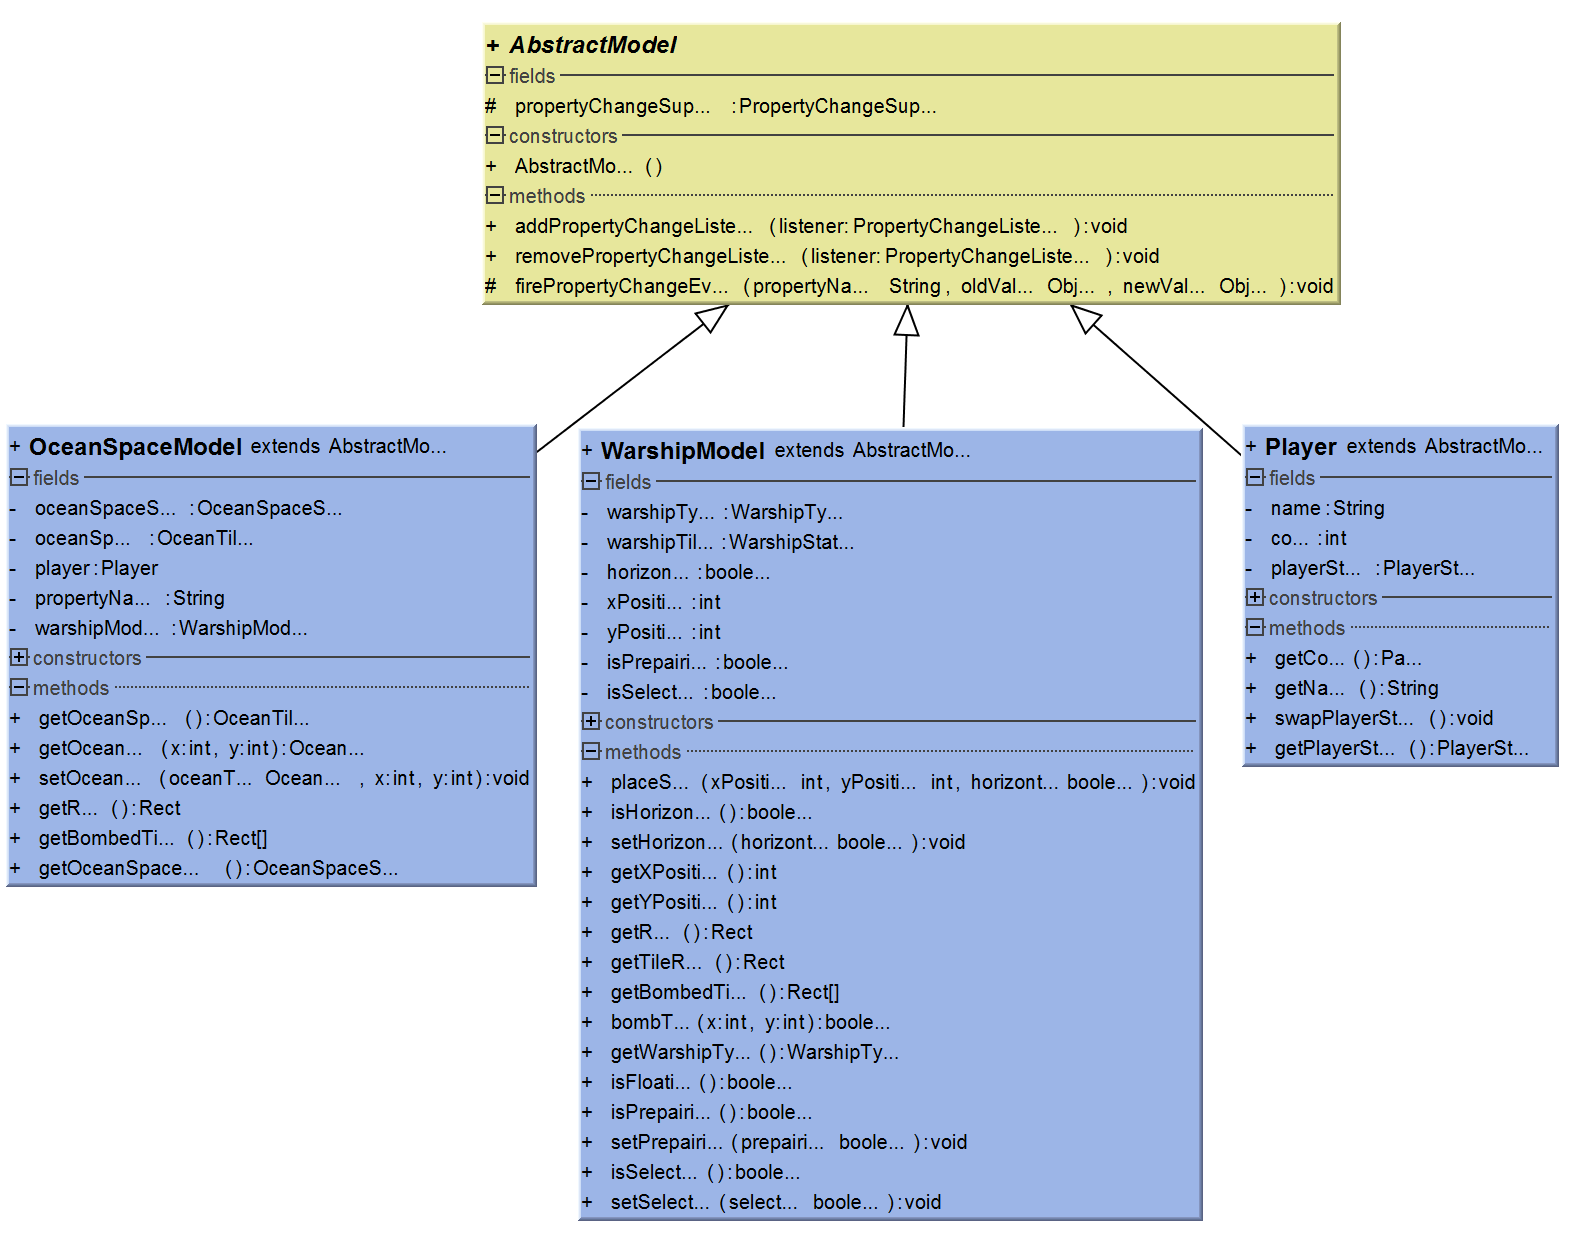
\includegraphics[width=\textwidth, angle=90]{img/Class_Model.png}
    \caption{Class diagram: Models}
    \label{fig:DevelopmentView}
\end{figure}

\begin{figure}[ht]
    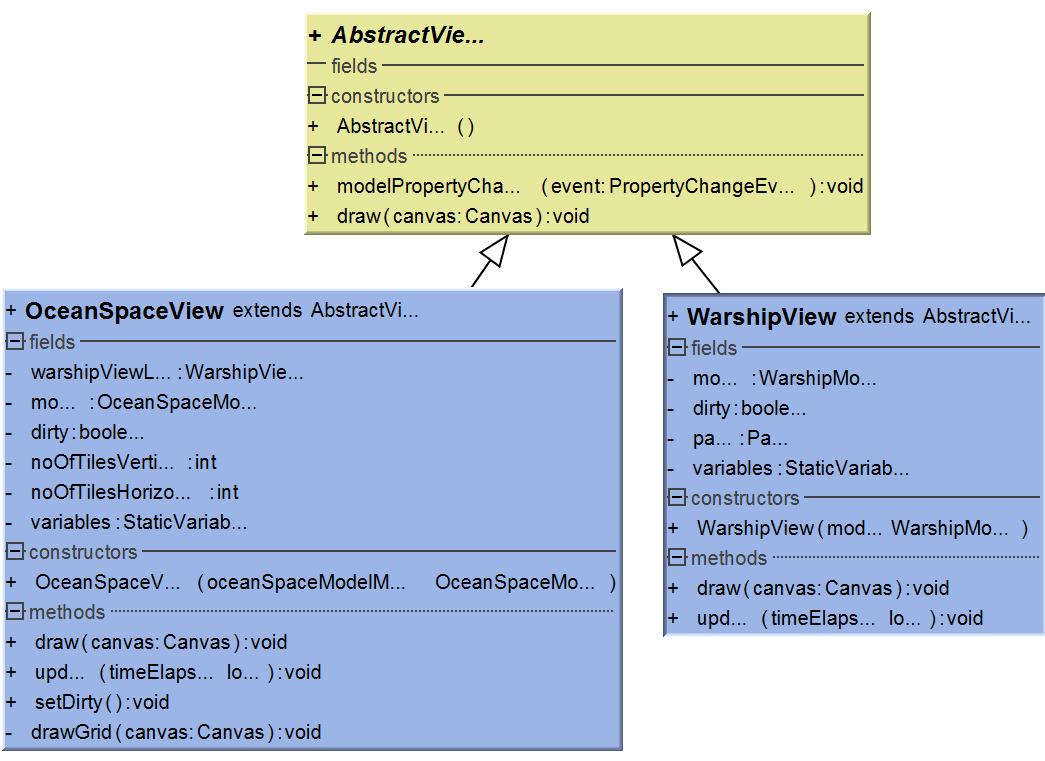
\includegraphics[width=\textwidth, angle=90]{img/Class_View.png}
    \caption{Class diagram: Views}
    \label{fig:DevelopmentView}
\end{figure}

\begin{figure}[ht]
    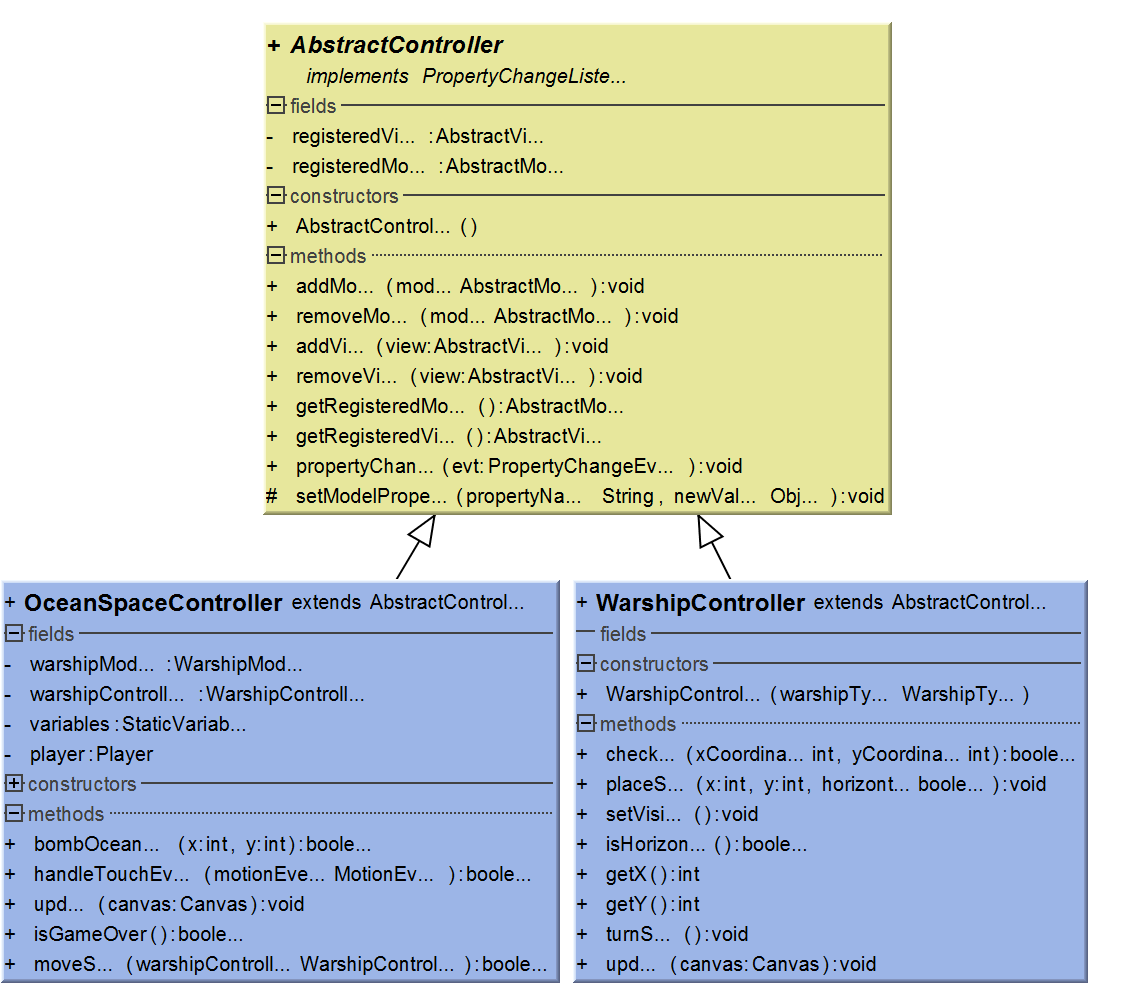
\includegraphics[width=\textwidth, angle=90]{img/Class_Controller.png}
    \caption{Class diagram: Controllers}
    \label{fig:DevelopmentView}
\end{figure}

\begin{figure}[ht]
    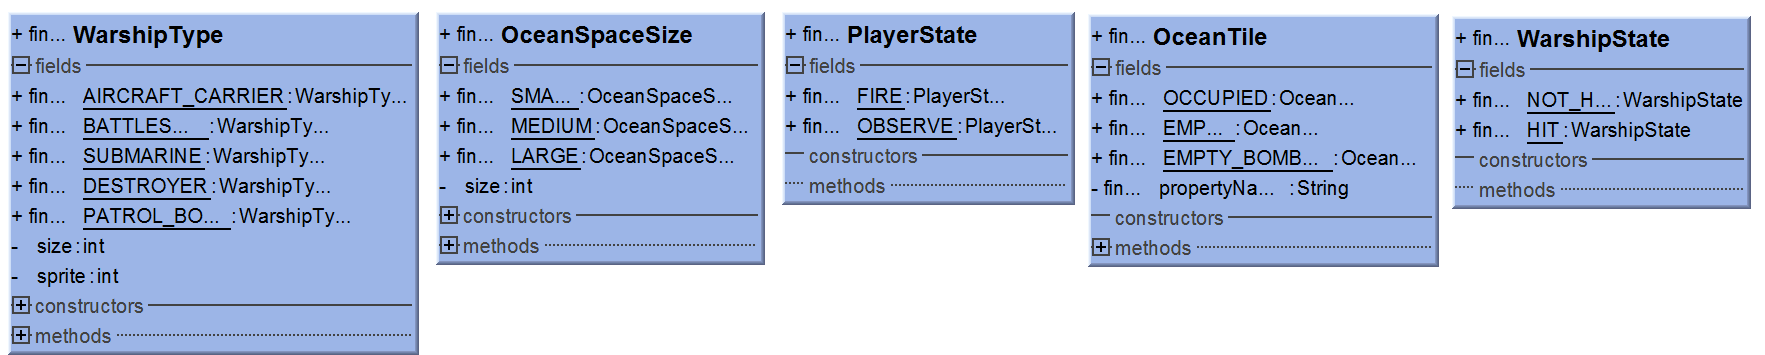
\includegraphics[width=\textwidth, angle=90]{img/Class_Enums.png}
    \caption{Class diagram: Enumerators}
    \label{fig:DevelopmentView}
\end{figure}

\begin{figure}[ht]
    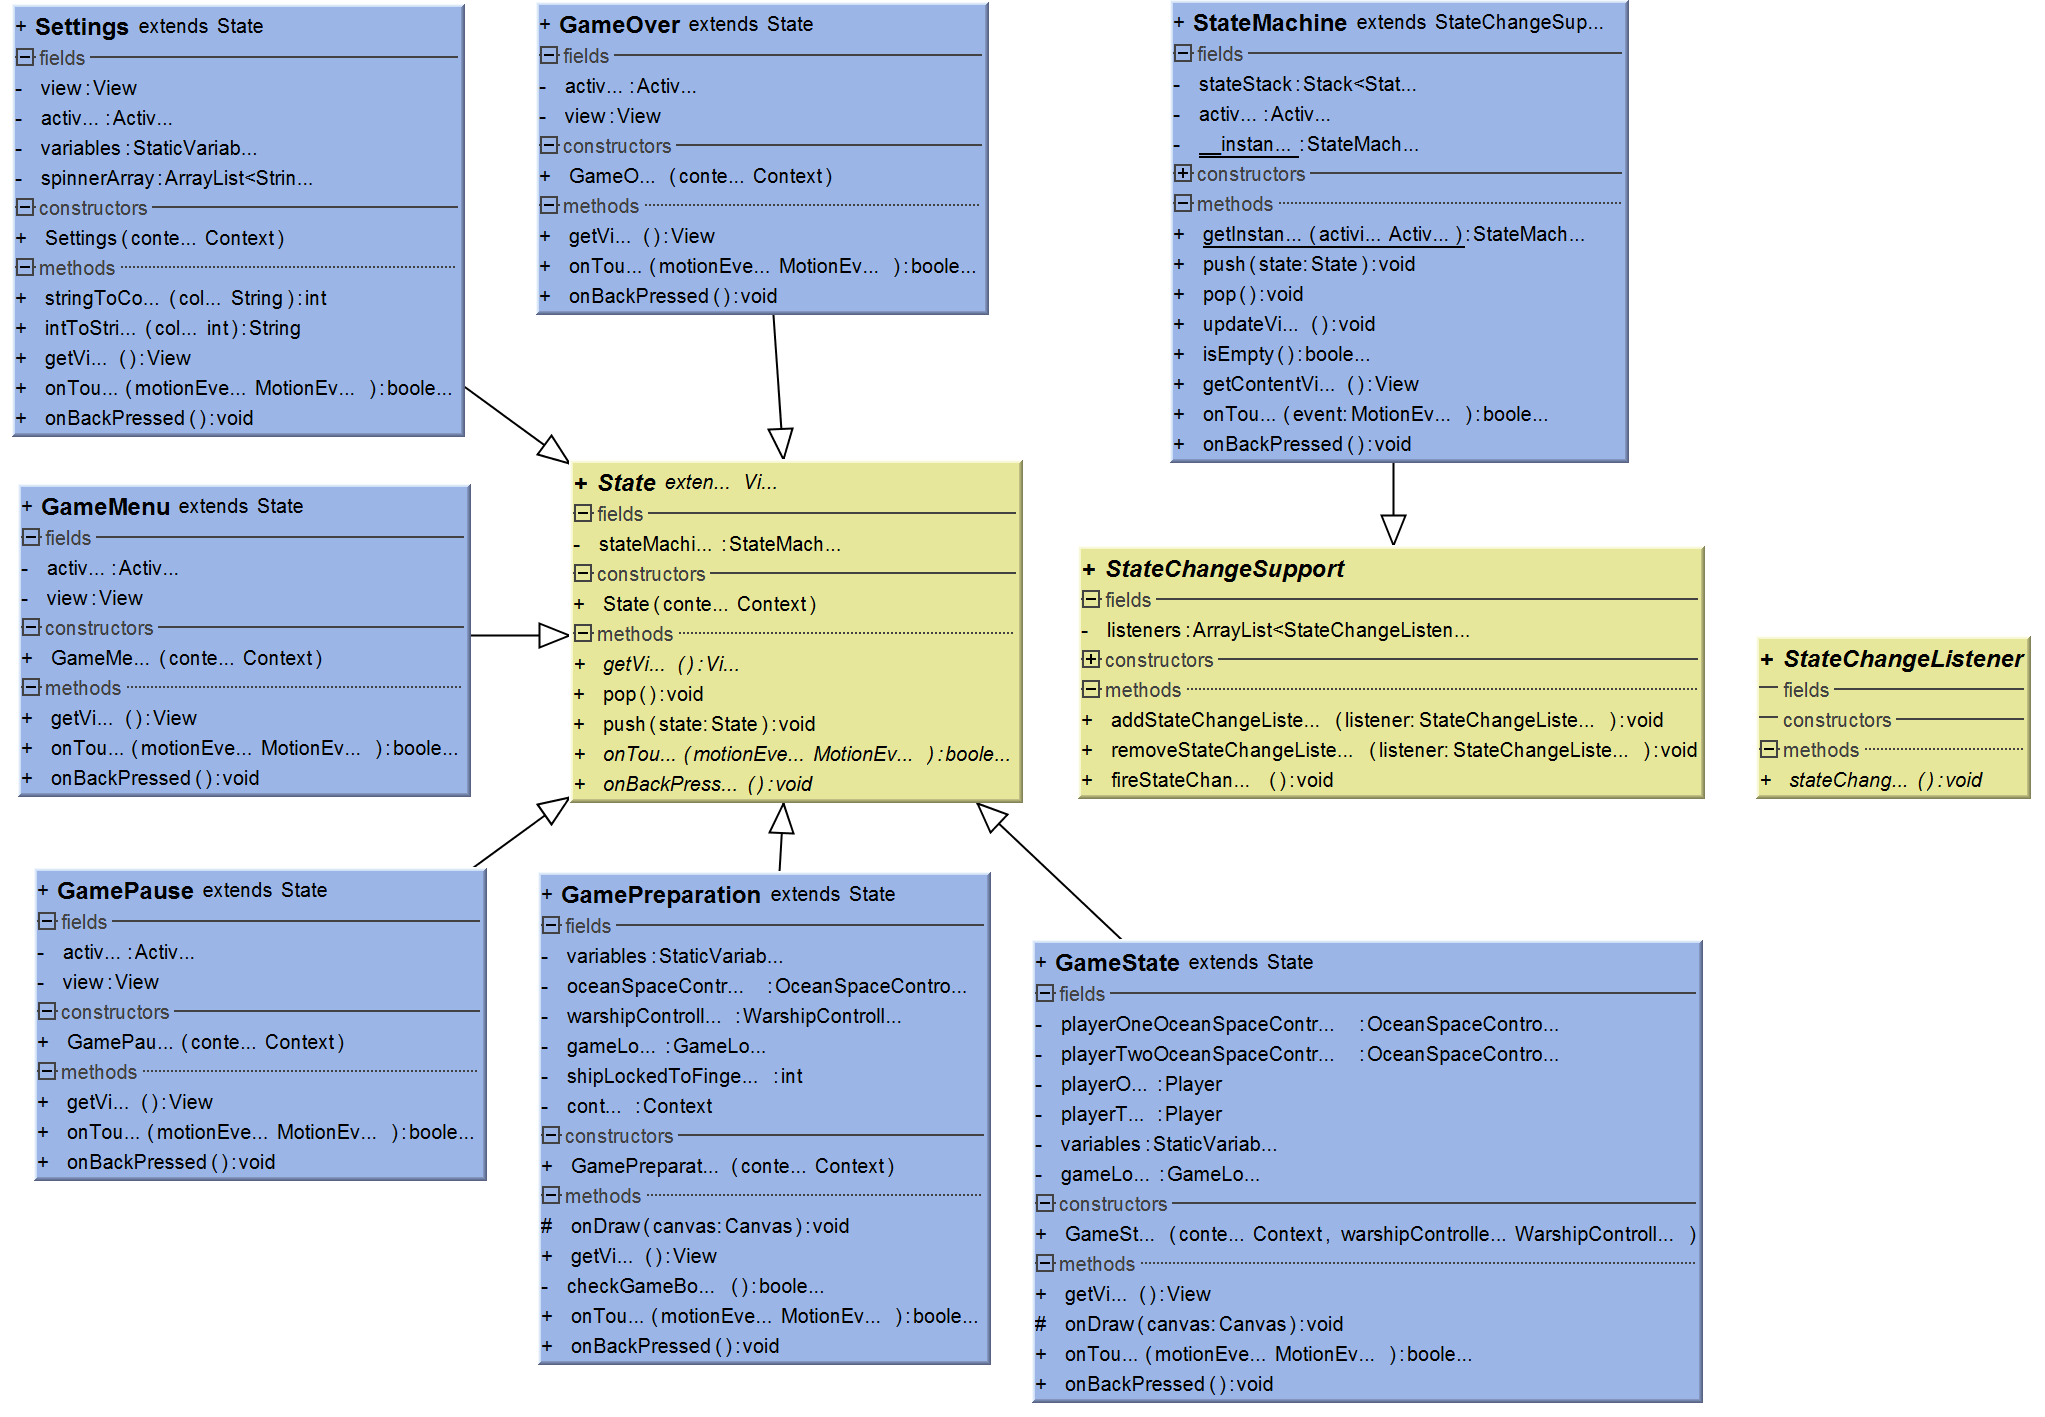
\includegraphics[width=\textwidth, angle=90]{img/Class_State.png}
    \caption{Class diagram: State}
    \label{fig:DevelopmentView}
\end{figure}

\begin{figure}[ht]
    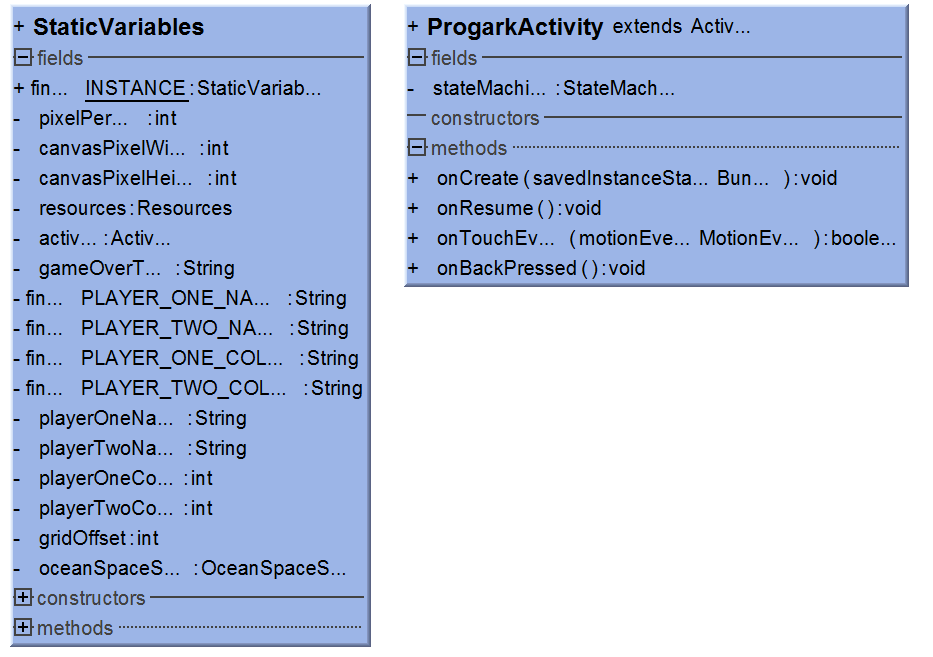
\includegraphics[width=\textwidth, angle=90]{img/Class_Misc.png}
    \caption{Class diagram: Miscellaneous}
    \label{fig:DevelopmentView}
\end{figure}